\documentclass[twocolumn]{article}
\usepackage[utf8]{inputenc}
\usepackage{amsmath} % Advanced math typesetting
\usepackage[utf8]{inputenc} % Unicode support (Umlauts etc.)
\usepackage[english]{babel} % Change hyphenation rules
\usepackage{hyperref} % Add a link to your document
\usepackage{graphicx} % Add pictures to your document
\usepackage{listings} % Source code formatting and highlighting
\usepackage{bookmark}
\usepackage{natbib}
\usepackage{geometry}
\usepackage{bbm}
%\usepackage{multicol}
\usepackage{fancyhdr}
\usepackage[document]{ragged2e}
\usepackage{adjustbox}
\usepackage{subcaption}
% \pagestyle{fancy}
% \fancyhf{}
% \fancyhead[LE,RO]{Overleaf}
% \fancyhead[RE,LO]{Guides and tutorials}
% \fancyfoot[CE,CO]{\leftmark}
% \fancyfoot[LE,RO]{\thepage}
\graphicspath{ {Immagini/} }
%C:\Users\erikz\OneDrive\Desktop\PaioPaio2\IMM-Sensors-Network\Latex\Immagini
\geometry{
 a4paper,
 total={170mm,257mm},
 left=20mm,
 top=20mm,
 }

\title{Report and analysis on implementation of IMM algorithm for multiple-model dynamics tracking}
\author{
Paiola Lorenzo 198573 

Zanolli Erik 198852}
\date{January 2020}





\begin{document}

\maketitle



\section*{Introduction}
\justify
The purpouse of this project is to analyze and evaluate the performance of an IMM algorithm's implementation in a distributed environment for
multiple-model dynamics tracking. The tracked agent switches between linked models of movement by the means of a Markov chain. The goal
is to evaluate the best trade-off between error on estimated position and real position and number of messages regarding consensus involved in the tracking.


\section*{Setting}
\justify
The general objective of this report is to provide a robust tracking that works in a distributed manner for some object that can move
in a number of different ways (modelized as a set of dynamical systems $\mathbbm{M}$). The environment in which this object moves is
one of a large room that contains multiple sensors that can talk to each other.
\\
\section*{Sensor's model}
\label{sensor}
The sensors chosen are radars measuring the polar cordinates relative to themselves at which the agent is collocated at the timestep, and
are disposed in a uniform square grid. In order to simulate the real workings of a sensor, range of measuremnt has been limited to the distance
between one sensor and the following one in any direction of the grid, as soon as the agent exceed the imposed maxiumum distance from the sensor,
the device will stop sensing.
This property of the sensor grid, coupled by its geometry, ensures that no more than 4 sensors can measure the agent position at any time,
so it made sense to let the sensors switch between 3 different states named ON, OFF and IDLE. This can be justified as a way to make the system
more power efficient and to avoid useless data stream towards sensors that aren't currently in range and sensing.
The sensor is modeled as a state machine as shown in figure \ref{fig:statemachine}
\\
\begin{figure}[h!]
    \centering
    \includegraphics[width=\columnwidth]{sensor_state_machine.png}
    \caption{State machine sensor}
    \label{fig:statemachine}
\end{figure}
\\
Sensors in different states differ between each other by the actions that are allowed in the state they are currently in.
\\
Here we enumerate such allowed actions:
\begin{itemize}
    \item ON: at each time-step checks if it is still in range with the function inRange(), takes a measurement, computes the IMM algorithm and
          at a tunable rate computes the consensus with the other nearby ON sensors. If it's not in range anymore then turns IDLE.
    \item IDLE : checks if it is now in range with the function inRange(), if it is then initialize itself with the data from nearby sensors
          that are ON. If it recieves a CantSense signal, it checks if at least one of its neighboors is still ON, else it turns OFF itself.
    \item OFF : does nothing but waits for a CanSense signal sent by a neighboor and turns IDLE in the case it has received one (this means that
          a nearby sensor has turned ON).
\end{itemize}
So sensors can communicate with the devices adjacent to them (Neighboorhood), as represented in the figure \ref{fig:neighboors} below,
and exchange with them signals named CanSense and CantSense which state respectively whenever the agent gets in or goes out of the
communicating sensor's range. This check is done through the function inRange() that also serves as a switch between the states of the
sensor, as already shown by the figure \ref{fig:statemachine} above.
The messages that the sensors exchange with their Neighboorhood are
\begin{itemize}
    \item CanSense : message sent by a sensor switching from IDLE to ON triggered by a positive result from InRange() function
    \item CantSense : message sent by a sensor switching from ON to IDLE triggered by a negative result from InRange() function
\end{itemize}
\begin{figure}[h!]
    \centering
    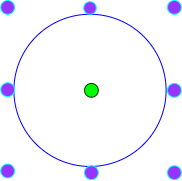
\includegraphics[width=0.2\textwidth]{Immagini/2sensor.png}
    \caption{The neighboors of a sensors are the one immediately adiacent, represented as purple in this image}
    \label{fig:neighboors}
\end{figure}
By defing the range of the sensors equal to their spacing on the grid it follows that only a maximum of 4 sensors can be turned on.
This fact is shown in the following picture that illustrates the different cases
\begin{figure}[h!]
    \centering
    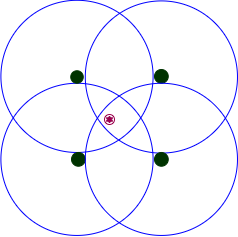
\includegraphics[width=0.23\textwidth]{Immagini/4sensor.png}
    \caption{}
    \label{fig:number}
\end{figure}
\begin{itemize}
    \item blue : 1 sensors ON
    \item yellow : 2 sensors ON
    \item orange : 3 sensors ON
    \item red : 4 sensors ON
\end{itemize}
Note that the blue case happens only at the borders and corners of the grid.
\\
Whenever the target is in range of a sensor at given timestep, the device takes a measurement.
The model choosen for our sensor is a Radar, and as such the non-linear measurement function
associated to it is the cartesian to polar transformation at timestep $k$, as shown below
\begin{align*}
     & z(k)=h(x(k))+v(k)          \\
     & \begin{bmatrix}
        \rho(k) \\ \theta (k)(k)
    \end{bmatrix}=
    \begin{bmatrix}
        \sqrt{x_{1}(k)^2+x_{2}(k)^2} \\ atan2(x_{2}(1)/x_{1}(k))
    \end{bmatrix} +
    \begin{bmatrix}
        v_{1}(k) \\v_{2}(k)
    \end{bmatrix}
\end{align*}
where $h(x)$ is the polar to cartesian cordinates transform that takes in $x(k)$ that is the state (of which the first 2 elements are the cartesian
cordinates relative to the sensor), $z(k)$ is the measure and $v(k)$ is the noise associated to the measurement's operation. The measurement noise $w(k)$ is associated
to a diagonal power spectral density matrix $R$.
\begin{equation*}
    R=\begin{bmatrix}
        \sigma^{2}_{\rho} & 0                       \\
        0                 & \sigma^{2}_{\theta (k)}
    \end{bmatrix}
\end{equation*}
\\
The matrix $H^{k}=(\nabla_{x} h(x))_{|x=x(k)}$ used in the linearized model with $v(k)=0$, necessary in the IMM filter at each timestep $k$,
computes to
\begin{equation*}
    H^{k}= \begin{bmatrix}
        \frac{x_{1}}{\sqrt{x_{1}^{2}+x_{2}^{2}}} & \frac{x_{2}}{\sqrt{x_{1}^{2}+x_{2}^{2}}} & 0 \dots \\
        \frac{-x_{2}}{x_{1}^{2}+x_{2}^{2}}       & \frac{x_{1}}{x_{1}^{2}+x_{2}^{2}}        & 0 \dots \\
    \end{bmatrix}_{|x=x(k)}
\end{equation*}
Where $0\dots$ is a vector of zeroes for all the other states that do not influence the measurement function.

\section*{Model used}
As mentioned already, the agent we want to track has a variable-model dynamic that can switch between different elements in a set
of models that we denote as $\mathbbm{M}$. We will consider 2 families of such sets that we will call: Random Accelerated Walk $\mathbbm{M}_{1}$
and Random Unicycle Turning $\mathbbm{M}_{2}$. Every element of said families is a discrete Markovian process, as all are influenced by a white
noise on their inputs.
\subsection*{Random Accelerated Walk}
For the Random Accelerated Walk we consider the set $\mathbbm{M}_{1}$ to be 5 elements large.
Here the elements are described
\begin{center}
    \begin{tabular}{||c||c |c |}%{|width=\columnwidth|}
        \hline
        Random Walk                         \\
        \hline\hline
        Mode   & Behaviour                  \\ [0.5ex]
        \hline\hline
        Mode 1 & Constant Speed             \\
        \hline
        Mode 2 & Positive Acceleration in x \\
        \hline
        Mode 3 & Negative Acceleration in x \\
        \hline
        Mode 4 & Positive Acceleration in y \\
        \hline
        Mode 5 & Negative Acceleration in y \\ [1ex]
        \hline
    \end{tabular}
\end{center}

Every member of the set has the same structure
to describe their dynamics, in state space this their shared linear model
\begin{equation}
    x(k+1)= Ax(k) + B(s_{k})u + Gw(k)
\end{equation}
where $A$ is the state matrix, $B(s_{k})$ the input matrix function of the mode/index $s_{k}$ that indicates the element picked of $\mathbbm{M}_{1}$ at timestep $k$,
$u$ is the input that stays constant at all timesteps $k$ and in all modes $s_{k}$, $G$ the noise matrix and $w(k)$ the process noise at timestep
$k$ with associated $Q_{1}$ diagonal power spectral density matrix.
\begin{equation*}
    Q_{1}=\begin{bmatrix}
        \sigma^{2}_{a_{x}} & 0                  \\
        0                  & \sigma^{2}_{a_{y}}
    \end{bmatrix}
\end{equation*}
Below we show the constant matrices and how the state is structured
\[ x=\begin{bmatrix} x \\ y \\ \dot{x} \\ \dot{y} \\ \end{bmatrix}  A=\begin{bmatrix}
        1 & 0 & \delta & 0      \\
        0 & 1 & 0      & \delta \\
        0 & 0 & 1      & 0      \\
        0 & 0 & 0      & 1      \\
    \end{bmatrix}
    G=\begin{bmatrix}
        \frac{\delta^{2}}{2} & 0                    \\
        0                    & \frac{\delta^{2}}{2} \\
        \delta               & 0                    \\
        0                    & \delta               \\
    \end{bmatrix}
\]
Where $x$ and $y$ are the cartesian coordinates in the absolute reference frame and $\delta$ is the duration of each timestep $k$.
To model different behaviours of the agent/elements in the set $\mathbbm{M}_{1}$ we use switching matrices $B(s_{k})$ while keeping the vector $u$
constant. The input $u$ here is a vector of acceleration in $x$ and $y$ that the noise $w(k)$ will influence.
We hypothesize that the input is always known in magnitude and constant. Here is the set $B(s_{k})$ of input matrices.
\begin{equation*}%[width=\columnwidth]
    \resizebox{.9 \columnwidth}{!}{
        $B(s_{k})=\begin{Bmatrix}
                \begin{bmatrix}
                    0 & 0 \\
                    0 & 0 \\
                    0 & 0 \\
                    0 & 0 \\
                \end{bmatrix}
                \begin{bmatrix}
                    \frac{\delta^{2}}{2} & 0 \\
                    0                    & 0 \\
                    \delta               & 0 \\
                    0                    & 0 \\
                \end{bmatrix}
                \begin{bmatrix}
                    -\frac{\delta^{2}}{2} & 0 \\
                    0                     & 0 \\
                    -\delta               & 0 \\
                    0                     & 0 \\
                \end{bmatrix}
                \begin{bmatrix}
                    0 & 0                    \\
                    0 & \frac{\delta^{2}}{2} \\
                    0 & 0                    \\
                    0 & \delta               \\
                \end{bmatrix}
                \begin{bmatrix}
                    0 & 0                     \\
                    0 & -\frac{\delta^{2}}{2} \\
                    0 & 0                     \\
                    0 & -\delta               \\
                \end{bmatrix}
            \end{Bmatrix} $
    }
\end{equation*}
\\
It is to note that the matrix $G$ is a merge between the second and the fourth matrices found in the set $B(s_{k})$ as we hyphotesized that
the noise will act randomly in direction and magnitude at every time-step.
\\
The jump between behaviours is modeled by a Markov chain that has a constant stochastic transition matrix $T$.
In the simulations the matrix is fixed at
\begin{equation*}
    T=\begin{bmatrix}
        p_{0} & p     & p     & p     & p     \\
        b     & q_{0} & 2q    & q     & 2q    \\
        b     & 2q    & q_{0} & 2q    & q     \\
        b     & q     & 2q    & q_{0} & 2q    \\
        b     & 2q    & q     & 2q    & q_{0} \\
    \end{bmatrix}
\end{equation*}
Where $p_{0}$, $q_{0}$ and $b$ are fixed while $p$ and $q$ are computed so that the matrix is stochastic.
\subsection*{Random Unicycle Turning}
In the case of the Random Unicycle Turning we also consider the set $\mathbbm{M}_{2}$ to be 5 elements large, but the states are changed.
\begin{center}
    \begin{tabular}{||c||c |c |}%{|width=\columnwidth|}
        \hline
        Unycicle                                        \\
        \hline\hline
        Mode   & Behaviour                              \\ [0.5ex]
        \hline\hline
        Mode 1 & Constant Tangential Velocity and Angle \\
        \hline
        Mode 2 & Positive Angular Wheel Acceleration    \\
        \hline
        Mode 3 & Negative Angular Wheel Acceleration    \\
        \hline
        Mode 4 & Positive Yaw Rate                      \\
        \hline
        Mode 5 & Negative Yaw Rate                      \\ [1ex]
        \hline
    \end{tabular}
\end{center}
Here all the elements in the set $\mathbbm{M}_{2}$ are non-linear models $x(k+1)=f(x(k),u(k),w(k),s_{k})$, but if we can still organize them in such a way
\begin{equation*}
    x(k+1)= A(x(k))x(k) + B(s_{k},x(k))u(k) + G(x(k))w(k)
\end{equation*}
By defining
\begin{equation*}
    \resizebox{.99\columnwidth}{!}{ $ x=\begin{bmatrix} x(k) \\ y(k) \\ v_{t}(k) \\ \alpha(k) \\ \end{bmatrix}
            A(x(k))=\begin{bmatrix}
                1 & 0 & \delta cos(\dot{\alpha (k)}) & 0                            \\
                0 & 1 & 0                            & \delta sin(\dot{\alpha (k)}) \\
                0 & 0 & 1                            & 0                            \\
                0 & 0 & 0                            & 1                            \\
            \end{bmatrix}
            G(x(k))=\begin{bmatrix}
                \frac{\delta^{2}}{2} cos(\alpha (k))r & 0      \\
                \frac{\delta^{2}}{2} sin(\alpha (k))r & 0      \\
                \delta r                              & 0      \\
                0                                     & \delta \\
            \end{bmatrix}
        $ } \end{equation*}
and
\begin{equation*}%[width=\columnwidth]
    \resizebox{.99 \columnwidth}{!}{
        $B(s_{k},k)=\begin{Bmatrix}
                \begin{bmatrix}
                    0 & 0 \\
                    0 & 0 \\
                    0 & 0 \\
                    0 & 0 \\
                \end{bmatrix}
                \begin{bmatrix}
                    \frac{\delta^{2}}{2} cos(\alpha (k))r & 0 \\
                    \frac{\delta^{2}}{2} sin(\alpha (k))r & 0 \\
                    \delta r                              & 0 \\
                    0                                     & 0 \\
                \end{bmatrix}
                \begin{bmatrix}
                    -\frac{\delta^{2}}{2} cos(\alpha (k))r & 0 \\
                    -\frac{\delta^{2}}{2} sin(\alpha (k))r & 0 \\
                    -\delta r                              & 0 \\
                    0                                      & 0 \\
                \end{bmatrix}
                \begin{bmatrix}
                    0 & 0      \\
                    0 & 0      \\
                    0 & 0      \\
                    0 & \delta \\
                \end{bmatrix}
                \begin{bmatrix}
                    0 & 0       \\
                    0 & 0       \\
                    0 & 0       \\
                    0 & -\delta \\
                \end{bmatrix}
            \end{Bmatrix} $
    }
\end{equation*}
where $\delta$ is the length of the timestep $k$, $r$ the radius of the unicycle's wheel, $x(k)$ and $y(k)$ absolute cartesian cordinates of the unicycle,
$v_{t}(k)$ tangential velocity and $\alpha$ yaw angle.
The input $u$ is a vector of the angular acceleration of the wheel $\omega$ and yaw rate $\Omega$ with
\begin{equation*}
    Q_{2}=\begin{bmatrix}
        \sigma^{2}_{\omega} & 0                   \\
        0                   & \sigma^{2}_{\Omega}
    \end{bmatrix}
\end{equation*}
Just as in $\mathbbm{M}_{1}$, $G$ is build on the hypothesis that the process noise $w(k)$ influences both inputs at any timestep $k$.
\\
The stochastic transition matrix in this case will be
\begin{equation*}
    T=\begin{bmatrix}
        p_{0} & p     & p     & p     & p     \\
        q     & q_{0} & q     & 0     & 0     \\
        q     & q     & q_{0} & 0     & 0     \\
        q     & 0     & 0     & q_{0} & q     \\
        q     & 0     & 0     & q     & q_{0}
    \end{bmatrix}
\end{equation*}
where $p_{0}$ and $q_{0}$ are fixed while $p$ and $q$ are computed to make the matrix stochastic.

\section*{IMM}
Being the agent's dynamic costantly switching between the models in the set chosen, a single Kalman filter won't give us acceptable results while
tracking and we have to rely on the Interacting Multiple Models algorithm (IMM). In essence the algorithm let various estimation filters work in parallel
(EKF in our case), and outputs a mixture of the filters' estimate based on the probability of each of the models used in the filter to be correct.
\\
The hyphotheses we have to make in order to use the IMM are that the sequence of the true mode at timestep $k$, $s_{k}$, is a Markovian process, i.e. the mode evolves to the
memoryless random process $P\{s_{k+1}^{(j)}|s_{k}^{(j)}\}\pi_{ji}$ $\forall\ j,i$ and that the model set $\mathbbm{M}$ is the correct one and is time-invariant.
In our case those hypotheses are known to be true.
\\
The design parameters of the IMM are the model set $\mathbbm{M}$, the process and measurement noise spectral density
matrices $Q$ and $R$ for each model and sensor, the initial state and covariance $\hat{x}_{0|0}$ and $P_{0|0}$
and the transition matrix $T$ containing all the $\pi_{ji}$.
\\
Following is a short recapof the algorithm, to see it in much more detail refer to %\cite%
\\
The algorithm can be subdivided in 4 subsections, :
\begin{itemize}
    \item Model Conditioned reinitialization $\forall m_{i},m_{j}\in \mathbbm{M}$
          \begin{align*}
               & \mu^{(i)}_{k|k-1}=\sum_{j}\pi_{ji}\mu^{(j)}_{k-1}                                              \\
               & \mu^{(j|i)}_{k-1}=\pi_{ji}\mu^{(j)}_{k-1}/\mu^{(i)}_{k|k-1}                                    \\
               & \bar{x}^{(i)}_{k-1|k-1}=\sum_{j}\hat{x}^{(j)}_{k-1|k-1}\mu^{j|i}_{k-1}                         \\
               & \bar{P}^{(i)}_{k-1|k-1}=\sum_{j}[P^{(j)}_{k-1|k-1}+(\bar{x}^{(i)}_{k-1|k-1}                    \\
               & -\hat{x}^{(j)}_{k-1|k-1})(\bar{x}^{(i)}_{k-1|k-1}-\hat{x}^{(j)}_{k-1|k-1})^{T}]\mu_{k-1}^{j|i}
          \end{align*}
          Here we take all the output model probabilities computed at the previous iteration of the IMM and mix them together with the
          transition matrix to then use the result to combine both the previous step state and covariance estimation. It is to 
          notice that the transpose of the matrix formed by the collection of $\mu^{(j|i)}_{k-1}$ is stochastic, this makes sense
          since it works as a normalized transition matrix while computing $\bar{P}^{(i)}_{k-1|k-1}$ and $\bar{x}^{(i)}_{k-1|k-1}$.
    \item Model Conditioned filtering $\forall m_{i}\in \mathbbm{M}$
          \begin{align*}
               & \hat{x}^{(i)}_{k|k-1}=f^{(i)}_{k}(\bar{x}^{(i)}_{k-1|k-1},u)                                                        \\
               & P^{(i)}_{k|k-1}=F^{(i)}_{k-1}\bar{P}^{(i)}_{k-1|k-1}F^{(i)^{T}}_{k-1}+G^{(i)}_{k-1}Q_{k-1}^{(i)}G^{(i)^{T}}_{k-1} \\
               & \bar{z}^{(i)}_{k}=z_{k}-h(\hat{x}^{(i)}_{k|k-1})                                                                  \\
               & S^{(i)}_{k}=H^{(i)}_{k}P^{(i)}_{k|k-1}H^{(i)^{T}}_{k}+R^{(i)}_{k}                                                 \\
               & W^{(i)}_{k}=P^{(i)}_{k|k-1}H^{(i)^{T}}_{k}S^{(i)^{-1}}_{k}                                                        \\
               & \hat{x}^{(i)}_{k|k}=\hat{x}^{(i)}_{k|k-1}+W^{(i)}_{k}\bar{z}^{(i)}_{k}                                            \\
               & P^{(i)}_{k|k}=P^{(i)}_{k|k-1}-W^{(i)}_{k}S^{(i)}_{k}W^{(i)^{T}}_{k}
          \end{align*}
          This part of the algorithm is the one that includes all the estimation filters running in parallel. In the case 
          of $\mathbbm{M}_{1}$ we use a Kalman filter with a non-linear $h(x)$, so $f^{(i)}_{k}(x,u)$ is just the linear model 
          $(i)$ inside $\mathbbm{M}_{1}$ while $F^{(i)}_{k-1}$ is $A$ and $G^{(i)}_{k-1}$ is $G$ specified in the model. In 
          $\mathbbm{M}_{2}$ case an Extended Kalman Filter is used since $f^{(i)}_{k}(x,u)$ is non-linear for every model $(i)$, 
          so here $F^{(i)}_{k-1}$ is the Jacobian of the non-linear function without noise evaluated in $\bar{x}^{(i)}_{k-1|k-1},\ u$ while 
          $G^{(i)}_{k-1}$ is $\nabla_{w}f^{(i)}_{k}(x,u)$ evaluated in the same point with noise$=0$. Both power spectral density 
          matrices $Q$ and $R$ are constant by assumption. The matrix $H^{(i)}_{k}$ will be model $(i)$ agnostic, computed 
          as already discussed in section \ref{sensor} and evaluated in $\hat{x}^{(i)}_{k|k-1}$ (each different sensor will 
          calculate its relative position from that coordinate).
    \item Model Probability update $\forall m_{i},m_{j}\in \mathbbm{M}$
          \begin{align*}
               & L^{(i)}_{k}=\mathcal{N}(\bar{z}^{(i)}_{k},0,S^{(i)}_{k})                                \\
               & \mu^{(i)}_{k}=\frac{\mu^{(i)}_{k|k-1}L^{(i)}_{k}}{\sum_{j}\mu^{(j)}_{k|k-1}L^{(j)}_{k}}
          \end{align*}
          Here we compute what is the actual probability of the model $m_{i}\in\mathbbm{M}$ to have guided the dynamic of 
          our agent at timestep $k$. To do so we assume that the the probability distribution of the error $\bar{z}_{k}$ should be 
          a Gaussian with $0$ mean and as covariance the innovation covariance $S^{(i)}_{k}$ given by the filter $(i)$ at timestep
           $k$, and we compute the $L^{(i)}_{k}$ probability density function in $\bar{z}^{(i)}_{k}$. Using this result we re-normalize the previously 
           computed $\mu^{(i)}_{k|k-1}$ to give us the output vector of model probabilities $\mu_{k}$.
           \\
           In this step a lower bound on the likelihood is implemented since a likelihood vector of $0$ breaks the algorithm.
    \item Estimate fusion
          \begin{align*}
               & \hat{x}_{k|k}=\sum_{i}x^{(i)}_{k|k}\mu^{(i)}_{k}                                                                      \\
               & P_{k|k}=\sum_{i}[P^{(i)}_{k|k}+(\hat{x}_{k|k}-\hat{x}^{(i)}_{k|k})(\hat{x}_{k|k}-\hat{x}^{(i)}_{k|k})^{T}]\mu_{k}^{i}
          \end{align*}
          Using the vector $\mu_{k}$ computed at the previous step we mix all of the predictions computed by the filters to get 
          the outputs. This last step is only for the sake of the output, the algorithm forms a loop without it.
\end{itemize}
\section*{Consensus}
Right after having computed the IMM's estimate for every ON sensor, we use a consensus algorithm to try to lower the
estimation error even more. The consensus will happen at a variable rate and only between the ON sensors.
The set of active sensors inside the grid is dynamic, as vertices keep getting added and popped. However no
more than 4 sensors will be ON at any point of time, see \ref{fig:number}, and they will all be adjacent to each other,
this let us model the graph of the active sensors as fully-connected, since the distance between them is short
and we imagine them to be directly linked.
\\
This modeling let us use a Weighted Least Squared estimation of the best measure between all the ON sensors, since this operation
gives us a consensus in a single timestep, which is what we need with both a dynamic graph and a dynamic system.
So for our system we get
\begin{align*}
     & P_{cons}(k)=(H^{k^{T}}P^{k^{-1}}H^{k})^{-1}  \\
     & x_{cons}(k)=P_{cons}H^{k^{T}}P^{k^{-1}}Z^{k}
\end{align*}
where $P^{k}$ is the block diagonal matrix built with all the covariance matrices from the IMM's output, $Z^{k}$
is the measurement vector built by stacking all the state predictions from the IMM's output and $H^{k}$ is the matrix build by
stacking all the $H_{i}$ for $z_{i}=H_{i}x+\epsilon_{i}$, luckily in our case all $H_{i}$ are identity matrices.\\
It has to be noted that the WLS can be seen as 2 parallel linear consensus algorithms, running one on top of the other.
The consensus is computed both on the output of the IMM filter and all the outputs of its internal Kalman filters.
\\
We also tentatively tried to use the same consensus algorithm on the prediction vector of model probabilities $\mu_{k}$ using
the collection of all $\mu^{j|i}_{k-1}$ in matrix form instead of the covariance matrix for the weighting matrix, but
the resulting matrix was too close to singularity and the simulation was having numerical problems so this road
was abandoned, instead we just computed the mean between the various $\mu_{k}$.
\newpage
\section*{Results}
Here we present the results of our implementation of the algorithm and sensors. The agent was left wandering inside the set virtual room 
and measured at each timestep the estimation error that the algorithm gave. The room is set to be a square with a $100m$ side with a $10\times 10$ 
grid of sensors with range$=10$. 
\\
The simulations were performed in a loop according to the Montecarlo's Method. We set a number of iterations for any specific case to 
$n_{monte}=100$ and each iteration stop wheter the agent leaves the room limits or a number of timesteps $n_{k}=1000$ is reached. The starting
 position and starting model are randomized at each iteration.
The performance indexes that we evaluated are:
\begin{itemize}
    \item The Root Mean Square of the means of the errors at each Montecarlo's iteration
    \item The Root Mean Square of the maximum error at every Montecarlo's iteration
    \item The Maximum error between all Montecarlo's iterations
\end{itemize}
We evaluated both model sets $\mathbbm{M}_{1}$ and $\mathbbm{M}_{2}$ for different consensus rate (how many timestep between each consensus), 
different $R$s and $Q$s and we considered both the errors given by the Consensus and by each individual sensor's IMM. 
\\
The timestep $\delta$ is set at $0.05s$, the radius of the wheel $r$ at $0.5m$ while the inputs are
\begin{align*}
    u_{1}=\begin{bmatrix}
        5\frac{m}{s^{2}} \\5\frac{m}{s^{2}}
    \end{bmatrix}\ \ \ \ 
    u_{2}=\begin{bmatrix}
        3\frac{rad}{s^{2}} \\6\frac{rad}{s}
    \end{bmatrix}
\end{align*}
The power spectral density matrices considered are $R1=diag(0.1,(\frac{2\pi}{180})^{2})$ and $R2=diag(0.01,(\frac{2\pi}{360})^{2})$ for all the sensors, 
and while $Q2=diag(1,1)$ is shared by $\mathbbm{M}_{1}$ and $\mathbbm{M}_{2}$, $Q1=diag(0.2,0.2)$ for $\mathbbm{M}_{2}$ and $Q1=diag(0.1,0.1)$ for $\mathbbm{M}_{1}$.
\\
The first case is $\mathbbm{M}_{1}$, the second $\mathbbm{M}_{2}$. Here are reported all the results of the simulations, all in meters.
%%%%%%%%%%%% SENSOR %%%%%%%%%%%%%%%%%%%

\begin{center}
    \resizebox{.99 \columnwidth}{!}{ $
            \begin{tabular}{ |c||c|c|c|  }
                \hline
                \multicolumn{4}{|c|}{Sensor}                 \\
                \hline
                Measure & RMS of Means & RMS of Maxes & Max of Maxes \\ [0.5ex]
                \hline
                R1,Q1   & 0.3985        & 1.2407       & 1.7790      \\
                \hline
                % R1,Q2           & 0.1132                &  0.2847           & 0.6577                      \\
                % \hline
                R2,Q1   & 0.1574        & 0.5454       & 0.7139      \\
                % \hline
                % R2,Q2           & 0.0539                & 0.1454             & 0.2334                   \\
                \hline
            \end{tabular} $}
\end{center}
This table is needed to compare the simulations results, because the power spectral density matrices $R$ regard the polar coordinates, while here
 we have the errors in cartesian. If the algorithm gives an error greater in all cases than what is given by the sensors, 
then it is useless.

\begin{center}
    \resizebox{.99 \columnwidth}{!}{ $
            \begin{tabular}{ |c||c|c|c|  }
                \hline
                \multicolumn{4}{|c|}{case 1: consensus rate = 20}      \\
                \hline
                Consensus & RMS of Means & RMS of Maxes & Max of Maxes \\ [0.5ex]
                \hline
                R1,Q1     & 0.1078        & 0.2578       & 0.3960      \\
                \hline
                R1,Q2     & 0.1094        & 0.2694       & 0.4671      \\
                \hline
                R2,Q1     & 0.0505        & 0.1210       & 0.2491      \\
                \hline
                R2,Q2     & 0.0514        & 0.1313       & 0.2549      \\
                \hline
                \multicolumn{4}{|c|}{}                                 \\
                \hline
                Individual IMM  & RMS of Means & RMS of Maxes & Max of Maxes \\
                \hline
                R1,Q1     & 0.1609        & 0.1762       & 2.0937      \\
                \hline
                R1,Q2     & 0.1625        & 0.1907       & 1.0347      \\
                \hline
                R2,Q1     & 0.0799        & 0.0877       & 0.4310      \\
                \hline
                R2,Q2     & 0.0815        & 0.0926       & 0.4445      \\
                \hline
            \end{tabular} $}
\end{center}


%%%%%%% rate 10 %%%%%


\begin{center}
    \resizebox{.99 \columnwidth}{!}{ $
            \begin{tabular}{ |c||c|c|c|  }
                \hline
                \multicolumn{4}{|c|}{case 1: consensus rate = 10}      \\
                \hline
                Consensus & RMS of Means & RMS of Maxes & Max of Maxes \\ [0.5ex]
                \hline
                R1,Q1     & 0.1110        & 0.2831       & 0.4460      \\
                \hline
                R1,Q2     & 0.1129        & 0.2940       & 0.5227      \\
                \hline
                R2,Q1     & 0.0516        & 0.1406       & 0.2226      \\
                \hline
                R2,Q2     & 0.0519        & 0.1331       & 0.2429      \\
                \hline
                \multicolumn{4}{|c|}{}                                 \\
                \hline
                Individual IMM  & RMS of Means & RMS of Maxes & Max of Maxes \\
                \hline
                R1,Q1     & 0.1455        & 0.1678       & 0.9         \\
                \hline
                R1,Q2     & 0.1478        & 0.1926       & 1.5835      \\
                \hline
                R2,Q1     & 0.0751        & 0.0853       & 0.4441      \\
                \hline
                R2,Q2     & 0.0756        & 0.0824       & 0.4522      \\
                \hline
            \end{tabular} $}
\end{center}



%%%%%%% rate 5 %%%%%
\begin{center}
    \resizebox{.99 \columnwidth}{!}{ $
            \begin{tabular}{ |c||c|c|c|  }
                \hline
                \multicolumn{4}{|c|}{case 1: consensus rate = 5}       \\
                \hline
                Consensus & RMS of Means & RMS of Maxes & Max of Maxes \\ [0.5ex]
                \hline
                R1,Q1     & 0.1158        & 0.3516       & 1.2838      \\
                \hline
                R1,Q2     & 0.1192        & 0.3245       & 0.5018      \\
                \hline
                R2,Q1     & 0.0553        & 0.1649       & 0.3532      \\
                \hline
                R2,Q2     & 0.0542        & 0.1649       & 0.2246      \\
                \hline
                \multicolumn{4}{|c|}{}                                 \\
                \hline
                Individual IMM  & RMS of Means & RMS of Maxes & Max of Maxes \\
                \hline
                R1,Q1     & 0.1302        & 0.2460       & 1.808       \\
                \hline
                R1,Q2     & 0.1359        & 0.1700       & 1.7787      \\
                \hline
                R2,Q1     & 0.0666        & 0.0762       & 0.762       \\
                \hline
                R2,Q2     & 0.0661        & 0.0738       & 0.4450      \\
                \hline
            \end{tabular} $}
\end{center}

%%%%%%% rate 2 %%%%%
\begin{center}
    \resizebox{.99 \columnwidth}{!}{ $
            \begin{tabular}{ |c||c|c|c|  }
                \hline
                \multicolumn{4}{|c|}{case 1: consensus rate = 2}       \\
                \hline
                Consensus & RMS of Means & RMS of Maxes & Max of Maxes \\ [0.5ex]
                \hline
                R1,Q1     & 0.1158        & 0.3516       & 1.2838      \\
                \hline
                % R1,Q2           & 0.1094                & 0.2694             & 0.4671                      \\
                % \hline
                R2,Q1     & 0.0598        & 0.1925       & 0.2654      \\
                % \hline
                % R2,Q2           & 0.0514                & 0.1313             & 0.2549                   \\
                \hline
                \multicolumn{4}{|c|}{}                                 \\
                \hline
                Individual IMM  & RMS of Means & RMS of Maxes & Max of Maxes \\
                \hline
                R1,Q1     & 0.1320        & 0.2460       & 1.808       \\
                \hline
                % R1,Q2           & 0.1625                & 0.1907             & 1.0347                     \\
                % \hline
                R2,Q1     & 0.0617        & 0.0741       & 0.4368      \\
                % \hline
                % R2,Q2           & 0.0815                & 0.0926            & 0.4445                   \\
                \hline
            \end{tabular} $}
\end{center}




%%%%%%% rate 1 %%%%%
\begin{center}
    \resizebox{.99 \columnwidth}{!}{ $
            \begin{tabular}{ |c||c|c|c|  }
                \hline
                \multicolumn{4}{|c|}{case 1: consensus rate = 1}       \\
                \hline
                Consensus & RMS of Means & RMS of Maxes & Max of Maxes \\ [0.5ex]
                \hline
                R1,Q1     & 0.4265        & 1.6287       & 4.5672      \\
                \hline
                % R1,Q2         & 0.0757                & 0.204             & 0.2612                        \\
                % \hline
                R2,Q1     & 0.0757        & 0.204        & 0.2612      \\
                % \hline
                % R2,Q2           & 0.0514                & 0.1313             & 0.2549                   \\
                \hline
                \multicolumn{4}{|c|}{}                                 \\
                \hline
                Individual IMM  & RMS of Means & RMS of Maxes & Max of Maxes \\
                \hline
                R1,Q1     & 0.3755        & 0.8706       & 5.9070      \\
                % \hline
                % R1,Q2           & 0.1625                & 0.1907             & 1.0347                     \\
                \hline
                R2,Q1     & 0.0766        & 0.1128       & 0.4872      \\
                % \hline
                % R2,Q2           & 0.0815                & 0.0926            & 0.4445                   \\
                \hline
            \end{tabular} $}
\end{center}




%%%%%%% no cons %%%%%
\begin{center}
    \resizebox{.99 \columnwidth}{!}{ $
            \begin{tabular}{ |c||c|c|c|  }
                \hline
                \multicolumn{4}{|c|}{case 1: consensus rate = 2}      \\
                \hline
                Individual IMM & RMS of Means & RMS of Maxes & Max of Maxes \\
                \hline
                R1,Q1    & 0.1790        & 0.2278       & 1.7442      \\
                \hline
                R1,Q2    & 0.1800        & 0.2782       & 6.4459      \\
                \hline
                R2,Q1    & 0.3961        & 0.0930       & 0.0850      \\
                \hline
                R2,Q2    & 0.0864        & 0.0973       & 0.7242      \\
                \hline
            \end{tabular} $}
\end{center}


%%%%%%%%%%%%%%%%%%%%%% 20 %%%%%%%%%%%%%%%%%
\begin{center}
    \resizebox{.99 \columnwidth}{!}{ $
            \begin{tabular}{ |c||c|c|c|  }
                \hline
                \multicolumn{4}{|c|}{case 2: consensus rate = 20}      \\
                \hline
                Consensus & RMS of Means & RMS of Maxes & Max of Maxes \\ [0.5ex]
                \hline
                R1,Q1     & 0.1167        & 0.3027       & 0.7750      \\
                \hline
                R1,Q2     & 0.1132        & 0.2847       & 0.6577      \\
                \hline
                R2,Q1     & 0.0512        & 0.1325       & 0.2315      \\
                \hline
                R2,Q2     & 0.0539        & 0.1454       & 0.2334      \\
                \hline
                \multicolumn{4}{|c|}{}                                 \\
                \hline
                Individual IMM  & RMS of Means & RMS of Maxes & Max of Maxes \\
                \hline
                R1,Q1     & 0.0771        & 0.0903       & 0.4918      \\
                \hline
                R1,Q2     & 0.1664        & 0.2726       & 1.0990      \\
                \hline
                R2,Q1     & 0.0771        & 0.0903       & 0.4918      \\
                \hline
                R2,Q2     & 0.0804        & 0.0947       & 0.4190      \\
                \hline
            \end{tabular} $}
\end{center}


%%%%%%%%%%%%%%%%% 10 %%%%%%%%%%%%%%%%%
\begin{center}
    \resizebox{.99 \columnwidth}{!}{ $
            \begin{tabular}{ |c||c|c|c|  }
                \hline
                \multicolumn{4}{|c|}{case 2: consensus rate = 10}      \\
                \hline
                Consensus & RMS of Means & RMS of Maxes & Max of Maxes \\ [0.5ex]
                \hline
                R1,Q1     & 0.1228        & 0.3438       & 0.5992      \\
                \hline
                R1,Q2     & 0.1214        & 0.3291       & 0.7441      \\
                \hline
                R2,Q1     & 0.0535        & 0.1536       & 0.2525      \\
                \hline
                R2,Q2     & 0.0539        & 0.1439       & 0.2396      \\
                \hline
                \multicolumn{4}{|c|}{}                                 \\
                \hline
                Individual IMM  & RMS of Means & RMS of Maxes & Max of Maxes \\
                \hline
                R1,Q1     & 0.1566        & 0.1938       & 0.8766      \\
                \hline
                R1,Q2     & 0.1577        & 0.2278       & 1.4168      \\
                \hline
                R2,Q1     & 0.0742        & 0.0906       & 0.3968      \\
                \hline
                R2,Q2     & 0.0759        & 0.0935       & 0.4782      \\
                \hline
            \end{tabular} $}
\end{center}

%%%%%%%%%%%%%%%%%%%%%%%%%%%% 555555 %%%%%%%%%%%%%%%%
\begin{center}
    \resizebox{.99 \columnwidth}{!}{ $
            \begin{tabular}{ |c||c|c|c|  }
                \hline
                \multicolumn{4}{|c|}{case 2: consensus rate = 5}       \\
                \hline
                Consensus & RMS of Means & RMS of Maxes & Max of Maxes \\ [0.5ex]
                \hline
                R1,Q1     & 0.1984        & 0.7467       & 2.3522      \\
                \hline
                R1,Q2     & 0.1925        & 0.5871       & 2.2983      \\
                \hline
                R2,Q1     & 0.0604        & 0.1829       & 0.4389      \\
                \hline
                R2,Q2     & 0.0628        & 0.1873       & 0.2912      \\
                \hline
                \multicolumn{4}{|c|}{}                                 \\
                \hline
                Individual IMM  & RMS of Means & RMS of Maxes & Max of Maxes \\
                \hline
                R1,Q1     & 0.2135        & 0.7295       & 2.4394      \\
                \hline
                R1,Q2     & 0.2116        & 0.5412       & 2.7371      \\
                \hline
                R2,Q1     & 0.0722        & 0.1012       & 0.4599      \\
                \hline
                R2,Q2     & 0.0742        & 0.1077       & 0.5699      \\
                \hline
            \end{tabular} $}
\end{center}

%%%%%%%%%%%%%%%%%%%%%%%%%       2          %%%%%%%%%%%%%%%%%%%%

\begin{center}
    \resizebox{.99 \columnwidth}{!}{ $
            \begin{tabular}{ |c||c|c|c|  }
                \hline
                \multicolumn{4}{|c|}{case 2: consensus rate = 2}       \\
                \hline
                Consensus & RMS of Means & RMS of Maxes & Max of Maxes \\ [0.5ex]
                \hline
                R1,Q1     & 0.6709        & 3.2770       & 8.4954      \\
                \hline
                % R1,Q2           & 0.1132                &  0.2847           & 0.6577                      \\
                % \hline
                R2,Q1     & 0.1392        & 0.6907       & 2.0562      \\
                % \hline
                % R2,Q2           & 0.0539                & 0.1454             & 0.2334                   \\
                \hline
                \multicolumn{4}{|c|}{}                                 \\
                \hline
                Individual IMM  & RMS of Means & RMS of Maxes & Max of Maxes \\
                \hline
                R1,Q1     & 0.07629       & 2.5799       & 9.3296      \\
                % \hline
                % R1,Q2        & 0.1664                & 0.2726                & 1.0990              \\
                \hline
                R2,Q1     & 0.1585        & 0.5868       & 2.1211      \\
                %     \hline
                %     R2,Q2           & 0.0804                & 0.0947            & 0.4190                   \\
                % \hline
            \end{tabular} $}
\end{center}


%%%%%%%%%%%%%%%%%%%% 1 1 1 %%%%%%%%%%%%%%%%%%%%%%%%%

\begin{center}
    \resizebox{.99 \columnwidth}{!}{ $
    \begin{tabular}{ |c||c|c|c|  }
        \hline
        \multicolumn{4}{|c|}{case 2: consensus rate = 1} \\
        \hline
        Consensus & RMS of Means & RMS of Maxes & Max of Maxes \\  [0.5ex]
        \hline
        R1,Q1    &      1.3654 & 5.5341 & 16.2066             \\
            \hline
             R2,Q1            & 0.3883                & 2.3273               & 5.1490                      \\
             \hline
        %     R2,Q1            & 0.0512                & 0.1325             & 0.2315                      \\
        %     \hline
        %     R2,Q2           & 0.0539                & 0.1454             & 0.2334                   \\
        % \hline
        \multicolumn{4}{|c|}{} \\
        \hline
        Individual IMM & RMS of Means & RMS of Maxes & Max of Maxes \\ 
        \hline
        R1,Q1      & 1.4520 & 5.6335 & 16.4740          \\
         \hline
        % R1,Q2        & 0.1664                & 0.2726                & 1.0990              \\
        % \hline
         R2,Q1         & 0.3867                & 1.3242             & 5.3175                         \\
        \hline
        % R2,Q2           & 0.0804                & 0.0947            & 0.4190                   \\
    \hline
       \end{tabular} $}
    \end{center}

%%%%% NO cons %%%%%%%%%%%%%%%%

\begin{center}
    \resizebox{.99 \columnwidth}{!}{ $
            \begin{tabular}{ |c||c|c|c|  }
                \hline
                \multicolumn{4}{|c|}{case 2: no consensus}                             \\
                \hline
                Individual IMM & RMS of Means & RMS of Maxes & Max of Maxes \\
                \hline
                R1,Q1    & 0.1784        & 0.2516       & 1.5541      \\
                \hline
                R1,Q2    & 0.1795        & 0.2145       & 0.9872      \\
                \hline
                R2,Q1    & 0.0845        & 0.0962       & 0.6888      \\
                \hline
                R2,Q2    & 0.0843        & 0.1090       & 0.9289      \\
                \hline
            \end{tabular} $}
\end{center}

What we gather from these tables is that, specifically in the case of the unicycle $\mathbbm{M}_{2}$ (that is a more complex model set), 
a consensus computed at a high frequency (rate=1, rate=2) gives disastrous results with any magnitude of noise. This is probably caused by 
the nature of the IMM algorithm that gets impeded by the consensus which homogenizes the internal Kalman filters input to a point which 
the IMM can't compute their probabilities efficiently. In fact we see a much better results with lower frequency such as rate=10 and rate=20.
We also tried the case in which we do not compute any consensus and we let individual sensors work alone and, while we see good results, 
it doesn't seem to be the best compromise.
\\
In the case of the Random Walk with a rate=2 we have good results with low $R$, but the algorithm is really sensible to changes to this 
parameter and performs really bad with $R1$.
\\
While we see that with both model sets the case with rate=20 gives very good results, but we also notice that the maximum of both the individual 
IMMs and of the consensus can get pretty high so if we have an application where the frequency of estimation must be high and we can't 
have a big overshoot, then this rate can fail.
All things considered the best compromise may be the rate=10, which always gives good results and has double the frequency of rate=20.
\\
Following are some graphs of the best and worst cases computed by the simulations. More graphs and a video of the algorithm working can 
be found at ... 

\end{document}
